%\documentclass[stu, 12pt]{apa7}
\documentclass[stu, 12pt, floatsintext]{apa7}
%\usepackage{fontspec}
%\setmainfont{Times New Roman} % Or your system's equivalent serif font
\usepackage[american]{babel}
\usepackage{csquotes}
\usepackage[style=apa, backend=biber]{biblatex}
%\usepackage[style=authoryear, backend=biber]{biblatex} % Changed from style=apa
\usepackage{float}
\usepackage{multicol}
\usepackage{hyperref} % nameref is bundled with hyperref
\usepackage{graphicx}   % Required for including images
\usepackage{subcaption} % Required for subfigures and subcaptions
%\usepackage{listings}
%\usepackage{xcolor}
\usepackage{array}
\usepackage{booktabs}
\usepackage{multirow}
\usepackage[dvipsnames]{xcolor}
\usepackage{amsmath}
\usepackage{amssymb}
\usepackage{enumitem,xcolor}

% Define the console style before using it
%\lstdefinestyle{console}{
	%	backgroundcolor=\color{black!5},
	%	basicstyle=\ttfamily\small,
	%	breaklines=true,
	%	frame=single,
	%	rulecolor=\color{black!30}
	%}
\graphicspath{
	{../img/}
	%   {../img_ipynb/}
	%	{../img/H1/}
	%	{../../results/DayResult/}
}
\DeclareGraphicsExtensions{.pdf,.jpeg,.png,.jpg}

\hypersetup{
	colorlinks=true,
	linkcolor=blue,
	citecolor=blue,
	urlcolor=blue
}

\addbibresource{../ref/references.bib}
\title{Industrial Equipment Anomaly \& Incident Response Agent}
\author{Max Raxy}
\affiliation{Udacity Institute of AI \& Technology}
\course{Capstone-6: Agentic AI Systems}
\professor{~}
\duedate{\today}

\begin{document}
	\maketitle
	\tableofcontents
	\newpage
	\listoffigures%\thispagestyle{fancy}
%	\listoftables%\thispagestyle{fancy}
	\newpage

\section{ALL}
We developed an agentic workflow~\parencites{agentic_Plaat_2025}{agentic_Hughes04072025} to classify pre-detected anomalies in industrial telemetry into three distinct operational response classes. The system identifies failure modes, performs root-cause analysis, suggests corrective actions, and automatically routes the incident to the appropriate tier for execution. Built using LangGraph~\parencite{langgraph_overview_2026}, the orchestration graph utilizes a \textbf{single} central LLM\footnote{Large Language Model}~\parencite{enwiki:LLM} at the core classifier node to manage reasoning as a ReAct\footnote{Reasoning and Acting}~\parencite{react} agent across the workflow.

\subsection{Monitored Telemetry Parameters}
The system evaluates four core telemetry metrics, representative of critical industrial assets like a Multistage Centrifugal Water Pump~\parencite{enwiki:cent-pump}:
\begin{enumerate}[font=\large\color{red}]
	\item \textbf{Temperature (temperature\_c):}  Monitored at bearings, lubrication loops, or process fluids to track thermal friction and cooling efficiency.
	\item \textbf{Vibration (vibration\_hz):} Tracks mechanical oscillations to detect shaft misalignment, rotor imbalance, or bearing degradation.
	\item \textbf{Pressure (pressure\_psi):}  Measures internal suction, discharge, or hydraulic line pressures.
	\item \textbf{Power (power\_kw):} Tracks real-time electrical power consumption to evaluate motor load and overall efficiency.
\end{enumerate}

\subsection{Incident Severity Classification}
\begin{enumerate}[font=\large\color{red}]\setcounter{enumi}{-1}
	\item \textbf{CLASS\_0 (Immediate Shutdown):}  Catastrophic failure or severe danger requiring instant asset shutdown (Critical).
	\item \textbf{CLASS\_1 (Automated Control):} Process drift or minor operational stress involving controllable single-telemetry anomalies (Moderate risk).
	\item \textbf{CLASS\_2 (Escalate to Onsite Engineer):} Physical degradation or mechanical faults involving complex, multi-telemetry anomaly combinations (High risk).
\end{enumerate}

\subsection{Simplified Domain Grounding via Severity Bands}
While a production deployment would ideally integrate Retrieval-Augmented Generation (RAG) using technical manuals, this implementation uses a deterministic threshold tool to convert raw numerical anomalies into standardized severity bands (Critically Low, Low, Normal, High, Critically High) as shown in Fig.~\ref{fig:sev-band}.

\begin{figure}[!tbh]
	\centering
	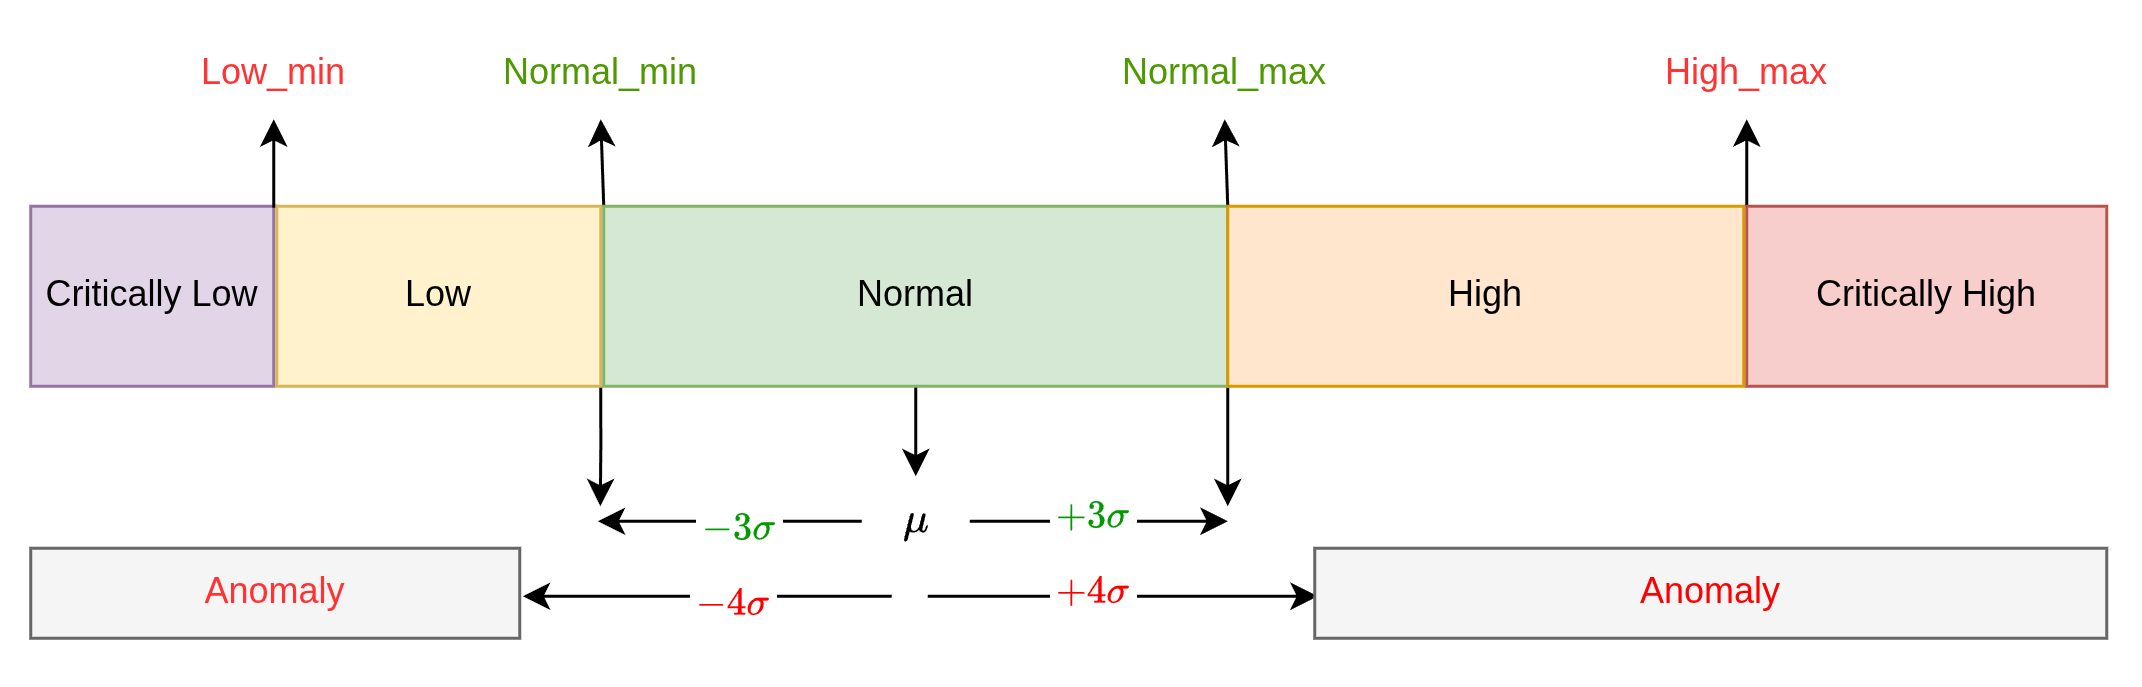
\includegraphics[width=1.0\textwidth]{severity_bands.drawio}
	\captionsetup{justification=centering}
	\caption{Severity Bands.}
	\label{fig:sev-band}
\end{figure}

Bypassing raw statistical metrics (e.g., standard deviations and means) prevents LLM hallucination and reasoning errors. This rule-based abstraction reflects practical engineering reality, where a variance of \textcolor{blue}{$10\sigma$} might represent a moderate operational shift in one metric(telemetry), but an immediate critical failure in another.

\subsection{Anomaly Detector}
It would be great to have a large dataset of the  real-world telemetry data labeled with normal and anomaly, and we could use Machine Leaning to build an anomaly detector. However in this project, this is not our goal, and we use a simple rule to detect anomaly data. As shown in Fig.~\ref{fig:sev-band}, we consider the full normal range as \textcolor{blue}{$6\sigma$} range with mean in the middle. Then if any telemetry is beyond  \textcolor{red}{$\pm4\sigma$} we consider it as anomaly. While the normal range is \textcolor{ForestGreen}{$\pm3\sigma$} , the gap ($[-4\sigma, -3\sigma]$ or $[+3\sigma, +4\sigma]$)  consider as tolerance beyond normal range before anomaly is reported.

\subsection{Workflow Graph}
The Graph for our agentic system is shown in Fig.~\ref{fig:graph}
\begin{figure}[!tbh]
	\centering
	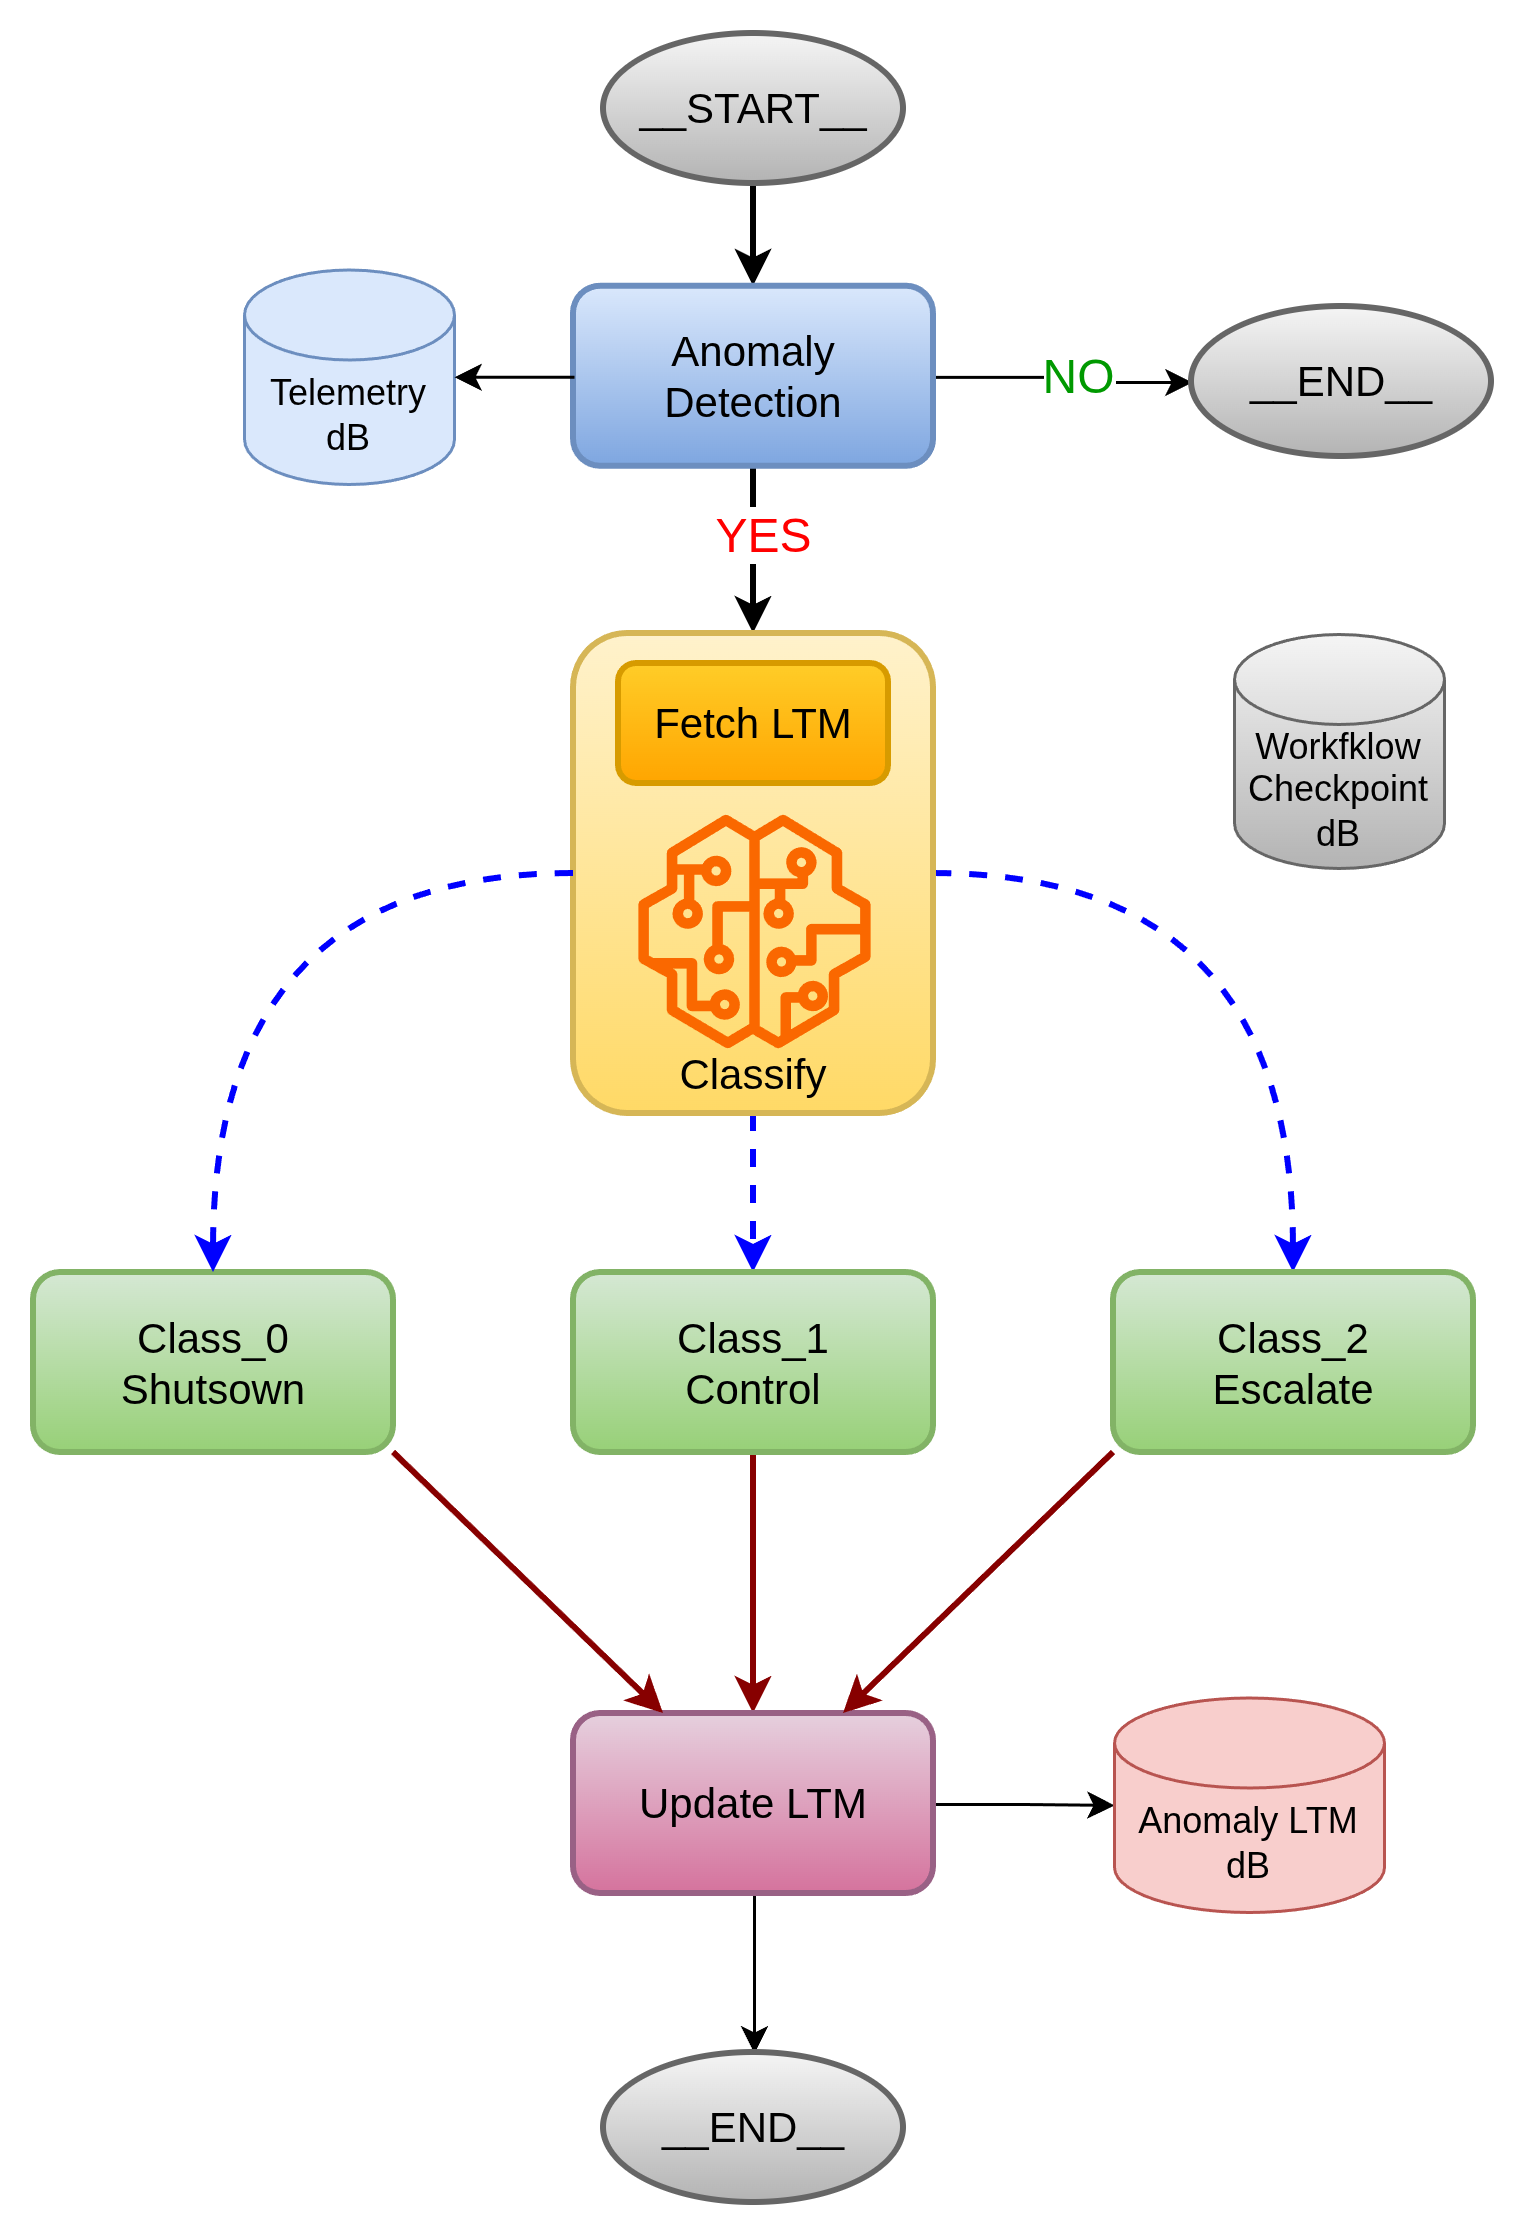
\includegraphics[width=0.5\textwidth]{workflow-details.drawio}
	\captionsetup{justification=centering}
	\caption{Workflow Graph.}
	\label{fig:graph}
\end{figure}
\begin{enumerate}[font=\large\color{red}]
	\item Telemetry data enter to anomaly detector node, it log to telemetry database, and if no anomaly detected, the workflow will end, otherwise it pass to the classifier Agent.
	\item Classifier agent is using
\end{enumerate}

\subsection{Note for later}
\begin{enumerate}
	\item we use checkpoint for audit and analytics on tool and token usage, the accumulated messages here is not used in agent so we do not need, sliding window, truncation or summarization
	\item Agent may need few previous long-term memory as context not the list of accumulated telemetry
	\item the response time is important for this agent, and while we could let agent to read LTM, we keep it out of agent tools, and we only let agent use one tool call to get severity bands
	\item class\_0 and class\_1 are clearly defined, and all other cases are escalate to human, as a future work we can add human in the loop for shutdown too, but if shutdown is critical may involving human delay the action, so it depends on the business if shutdown is too costly, and human decision is really needed
	\item In reality when CLASS\_1 send control command for increasing or decreasing a telemetry we will have close loop control, and here we did not have any simulation for it, and can be a part of future work
\end{enumerate}

\subsection{summary from my notebook}
1. We defined Norman and Anomaly Range
2. We defined the agentic workflow with one ReAct-agent (with one tool) and other nodes (python function that can be extended with ReAct-agent if required)
3. We define 3 assets (Multistage Centrifugal Water Pump) with their normal and anomaly ranges for 4 selected telemetries (temperature_c, vibration_hz,pressure_psi,power_kw)
4. We define 3 anomaly cases per asset to cover all anomaly classes (CLASS_0: Immediate Shutdown, CLASS_1: Automatic Adjust, and CLASS_2: Escalate)
5. We simulate each telemetry changes from start to end point, using sigmoid-like curve for better visual illustration (we can do linear change too, in our provided function)
6. Generally we use 2 sample for test , first in normal range, and the second in anomaly range (we can select more sample and see behavior as illustrated)
7. We tested all 9 test cases, with graph and snapshot of console, where all behave as expected
8. We try to fill Long-Term Memory (LTM) with same anomaly failure of CLASS_1, and agent switch its behavior to CLASS_2 which make sense, if Control is not effective better to escalate
9. Several day later we try same scenario again, and w expect to see CLASS_2, but agent tried CLASS_1 once then switch to CLASS_2, this might looks or considered as inconsistent decision by agent (specially with Temperature=0), but also can be consider smart decision that agent try to give a chance with automatic control then escalate again.
10. Overall since we clearly mentioned in our prompt, all unclear scenario escalate to On-Site Engineer and agent will not take action
11. We have 3 database (we used SQlite to make sure code is portable without requirement of additional setup for database)
12. Telemetry database that log all telemetry data
13. Short-Term Memory (STM) the checkpoint which mainly used for offline auditing and extracting analytic on tool/function calls and token usage
14. Long-Term Memory (LTM) to provide anomaly history for each asset as the context for agent action
15. Due to the nature of this work we did not need to use technique like sliding-window, summarization, or truncation on input messages to the agent, agent will take action on the current telemetry, plus the corresponding anomaly history ( generally last 3) from LTM which make the input (size) very controlled and deterministic.
16. There are many area that it can be improve or extend in this project including:
    - Use real dataset and develop a machine learning model for anomaly detection instead of simple python logic used in our anomaly detector
    - Use real test-data for anomaly test, or build a generative-AI to generate anomaly and normal data for test
    - We only use Variable Frequency Drive(VFD) for automatic control, while there are other parameter that can be controlled automatically (e,g. to reduce the pressure we may use opening a Bypass / Recirculation Valve)
    - When we have automatic control, we can add close loop control, to simulate reducing or increasing parameter, so system and agent see the real effect of the action taken


\section{Overview}
Explain the agentic task, system goal, and overall approach.

\section{System Architecture and Design}
Describe the agent’s components, reasoning flow, memory handling, and tool use. Include or reference your architecture diagram.

\section{Decision Logic and Behavior}
Explain how the agent makes decisions and how it responds to different inputs or situations.

\section{Safety, Reliability, and Transparency}
Discuss safeguards, constraints, and design choices intended to improve reliability, interoperability, or transparency.

\section{Observed Behavior and Limitations}
Analyze actual agent behavior based on your runs, including failure cases or limitations.

\section{Ethical and Responsible Use Considerations}
Identify at least one ethical concern related to autonomy, misuse, bias, accountability, or societal impact, grounded in your system’s design and behavior.

\section{Future Improvements}
Describe realistic next steps that could improve robustness, safety, or capability.


%---------------------------------------
Citation Requirements
\parencite{enwiki:dev-cent-pump}
Use citations when:

    Defining agentic AI concepts or architectures
    Justifying design patterns or safeguards
    Discussing ethical, governance, or responsible-use considerations

Do not cite your own code or execution outputs.
% apa does not include ref and appx in TOC we forced it
\phantomsection % Ensures hyperref links to the correct page
\addcontentsline{toc}{section}{References}
\printbibliography %[heading=none] % Removes default unnumbered header so it doesn't double-up

% Appendices start here (AFTER references)
%\appendix
%\phantomsection
%\addcontentsline{toc}{section}{Appendix A: Evaluation Metrics for Binary Classification}
%\section{Appendix A: Evaluation Metrics for Binary Classification}\label{app:a}
%\subsection{ELBO}
%Well,
%\newpage
%
%\phantomsection
%\addcontentsline{toc}{section}{Appendix B: XXX}
%\section{Appendix B: XXX}
%Content of Appendix B...
\end{document}